\documentclass{article}
\usepackage[spanish]{babel}
\usepackage[onehalfspacing]{setspace}
\usepackage[utf8]{inputenc}
\usepackage{amsmath}
\usepackage{amssymb}
\usepackage{verbatim}
\usepackage{graphicx}
\usepackage{listings}
\usepackage{fullpage}
\usepackage{color}
\usepackage{fancyvrb}
\usepackage{hyperref}
\hypersetup{%
	pdfborder = {0 0 0}
}

\definecolor{mygreen}{rgb}{0,0.6,0}
\definecolor{mygray}{rgb}{0.5,0.5,0.5}
\definecolor{mymauve}{rgb}{0.58,0,0.82}

\lstset{ %
	backgroundcolor=\color{white},   % choose the background color; you must add \usepackage{color} or \usepackage{xcolor}
	basicstyle=\footnotesize,        % the size of the fonts that are used for the code
	breakatwhitespace=false,         % sets if automatic breaks should only happen at whitespace
	breaklines=true,                 % sets automatic line breaking
	captionpos=b,                    % sets the caption-position to bottom
	commentstyle=\color{mygreen},    % comment style
	frame=single,                    % adds a frame around the code
	keepspaces=true,                 % keeps spaces in text, useful for keeping indentation of code (possibly needs columns=flexible)
	numbers=left,                    % where to put the line-numbers; possible values are (none, left, right)
	numbersep=5pt,                   % how far the line-numbers are from the code
	numberstyle=\tiny\color{mygray}, % the style that is used for the line-numbers
	rulecolor=\color{black},         % if not set, the frame-color may be changed on line-breaks within not-black text (e.g. comments (green here))
	showspaces=false,                % show spaces everywhere adding particular underscores; it overrides 'showstringspaces'
	showstringspaces=false,          % underline spaces within strings only
	showtabs=false,                  % show tabs within strings adding particular underscores
	stepnumber=1,                    % the step between two line-numbers. If it's 1, each line will be numbered
	stringstyle=\color{mymauve},     % string literal style
	tabsize=4,
	title=\lstname                   % show the filename of files included with \lstinputlisting; also try caption instead of title
}


\author{José Luis Cánovas Sánchez\\joseluis.canovas2@um.es\\48636907A}
\title{ARQUITECTURAS DE REDES AVANZADAS\\PRÁCTICA 1\\ ENERO 2015}
\date{}
\begin{document}
\maketitle

\begin{abstract}
	En este informe se redacta el desarrollo usando la herramienta GNS3 para el despliegue del escenario de red IPv6 con movilidad.
	%TODO: terminar
\end{abstract}

\tableofcontents
\section{Topología inicial}
Partimos en este proyecto creando una nueva topología en GNS3 equivalente a la del enunciado y que se puede ver en la imagen inferior. Para los routers se utiliza la ios del modelo C7200 de CISCO, con soporte para IPv6. Para los hosts, una imagen linux sin interfaz gráfica y con gestor de paquetes para poder instalar el soporte de mobile IPv6.\par

\begin{center}
	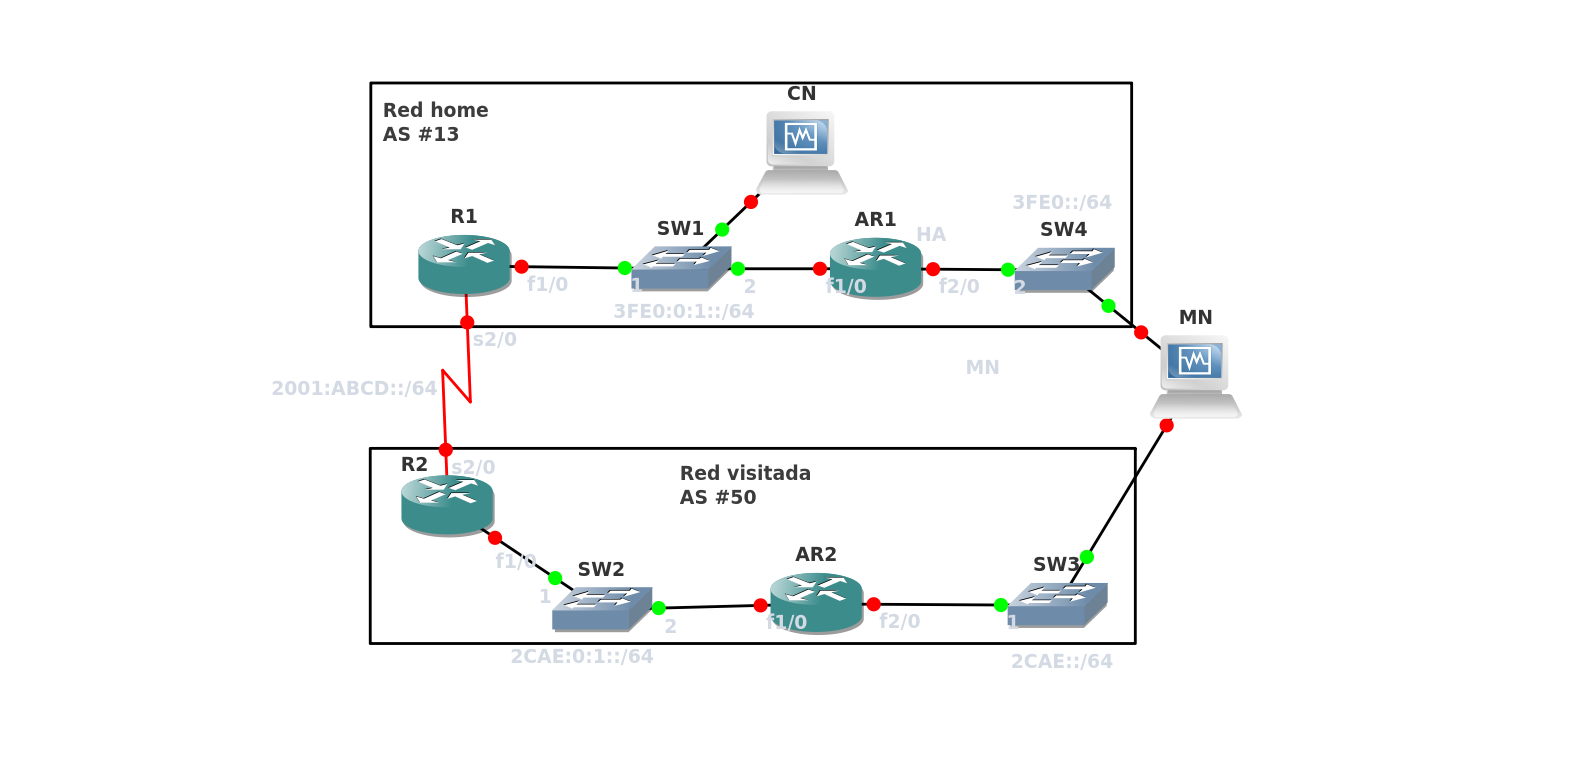
\includegraphics[scale=0.5]{images/topologyInic.png}
\end{center}

La configuración básica para que todos los dispositivos y redes tengan conectividad IPv6 entre ellas se puede realizar por medio del fichero de configuración del router directamente, y su equivalente en comandos de la terminal suelen ser las mismas líneas aplicadas en el nivel \textit{configure terminal}. En cuanto a los hosts, como utilizan la autoconfiguración de IPv6 no hace falta configurar manualmente nada.
\\

Veamos primero la configuración común de todos los routers:

Para activar IPv6 es necesario indicarlo antes de la configuración de las interfaces con \textit{ipv6 unicast-routing}. En cada interfaz que activemos, debemos indicar \textit{ipv6 enable} y la orden \textit{ipv6 address diripv6}, donde \textit{diripv6} es la dirección IPv6 asignada manualmente, o el prefijo de red seguido de \textit{eui-64} para permitir que la interfaz se autoconfigure su dirección.

Con esto tendríamos activado IPv6 en cada router, pero al intentar hacer \textit{ping} a una interfaz de otra red, vemos que no se recibe respuesta. Esto es porque no hay información en las tablas de rutas más que de las redes conectadas directamente a las interfaces de cada router.

Para cada Sistema Autónomo vamos a usar OSPF con soporte de IPv6. El diseño será de una única área 0 para todo el AS, lo que incluye las subredes en AS\#13 3FE0:0:1::/64 y 3Fe0::/64, y en AS\#50 las subredes 2CAE:0:1::/64 y 2CAE::64. Para ello, debemos activar OSPF en las dos interfaces de los routers AR1 y AR2, y en la interfaz FastEthernet1/0 de los routers R1 y R2 que se pueden ver en la figura de la topología más arriba.

Las órdenes para activar OSPF en cada router son:

Dentro de una interfaz que deba soportar OSPF (está dentro del área 0):
\begin{lstlisting}
ipv6 ospf 100 area 0
\end{lstlisting}

Tras la configuración de las interfaces:
\begin{lstlisting}
ipv6 router ospf 100
	router-id a.b.c.d
\end{lstlisting}

Donde \textit{a.b.c.d} es un valor identificador del router con 32 bits que se puede escribir como una dirección IPv4. Para cada router hemos elegido los identificadores \textit{1.1.1.1}, \textit{2.2.2.2}, \textit{3.3.3.3} y \textit{4.4.4.4} para R1, R2, AR1 y AR2 respectivamente. El valor 100 es indicador del proceso OSPF en el router y puede tomar cualquier otro valor, el tomar 100 es arbitrario.

Llegados a este punto, tenemos conectividad dentro de cada área, de modo que ahora un ping desde R1 a la interfaz de AR1 en la subred 3FE0::/64 funciona, pero de AR1 a R2 o AR2 no, porque no se conoce la ruta. Ahora mismo sólo R1 y R2 podrían hacer ping a las interfaces de la red 2001:ABCD::/64.

Para solucionarlo la forma más rápida es añadir una ruta estática en R1 y R2 a las redes del otro AS con la línea: \textit{ipv6 route 2CAE::/42 Serial2/0} en R1, y la equivalente \textit{ipv6 route 3FE0::/42 Serial2/0} en R2. Finalmente, en la configuración de OSPF, tras el \textit{router-id} añadimos la línea \textit{redistribute static}, sólo en R1 y R2, para que comuniquen con LSA5 (rutas fuera de dominio) que para alcanzar el otro AS a través de ellos hay una ruta.
\\

Ahora sí se puede realizar un ping desde cualquier dispositivo a cualquier otro, una vez OSPF ha convergido y compartido todos los mensajes. Pero como la mejora para configurar BGP entre R1 y R2 sobrescribe la configuración estática, mostraré las pruebas en el apartado siguiente.


\section{Configuración opcional BGP}
En los routers R1 y R2 debemos comentar o borrar las líneas de las rutas estáticas y su distribución en OSPF. A continuación, tras la configuración de OSPF podemos escribir la de BGP:
\\

Para R1:
\begin{lstlisting}
router bgp 13
	bgp router-id 1.1.1.1
	no bgp default ipv4-unicast
	!--- Without configuring ""no bgp default ipv4-unicast"" only IPv4 will be !--- advertised
	bgp log-neighbor-changes
	neighbor 2001:ABCD::2 remote-as 50
!
address-family ipv6
	neighbor 2001:ABCD::2 activate
	network 3FE0:0:1::/64
	network 3FE0::/64
exit-address-family
\end{lstlisting}

Donde 13 indica el número de Sistema Autónomo y 1.1.1.1 es un identificador equivalente al de OSPF, en este caso elegimos el mismo. La línea \textit{no bgp default ipv4-unicast} es necesaria para permitir las rutas con IPv6. La primera línea de \textit{neighbor} indica que en la interfaz de dirección 2001:ABCD::2, que corresponde a la IPv6 fija de R2, se encuentra el AS 50. A continuación, en el bloque \textit{address-family} activamos dicho vecino e indicamos que se deben anunciar las redes 3FE0:0:1::/64 y 3FE0::/64, correspondientes a las del AS 13 de la topología dada.

Para R2 la configuración sería equivalente cambiando los valores del 13 a 50 para el AS, el del \textit{router-id}, la dirección de R1 y las subredes a compartir.
\\

Con esto R1 y R2 conocerían las redes de cada AS, pero AR1 y AR2 todavía no, pues no hablan BGP. Sin embargo, sí hablan OSPF y añadiendo la línea en R1 y R2 \textit{redistribute bgp 10} en la configuración de OSPF (donde antes \textit{redistribute static}) se comunicarán las rutas externas con métrica 10 a los routers de cada AS. Podemos observarlo en la tabla de rutas de AR2, por ejemplo:

\begin{lstlisting}
Router>show ipv6 route
IPv6 Routing Table - 8 entries
Codes: C - Connected, L - Local, S - Static, R - RIP, B - BGP
U - Per-user Static route
I1 - ISIS L1, I2 - ISIS L2, IA - ISIS interarea, IS - ISIS summary
O - OSPF intra, OI - OSPF inter, OE1 - OSPF ext 1, OE2 - OSPF ext 2
ON1 - OSPF NSSA ext 1, ON2 - OSPF NSSA ext 2
C   2CAE::/64 [0/0]
via ::, FastEthernet2/0
L   2CAE::C801:1AFF:FE5F:38/128 [0/0]
via ::, FastEthernet2/0
C   2CAE:0:1::/64 [0/0]
via ::, FastEthernet1/0
L   2CAE:0:1:0:C801:1AFF:FE5F:1C/128 [0/0]
via ::, FastEthernet1/0
OE2  3FE0::/64 [110/2]
via FE80::C803:1AFF:FE5F:1C, FastEthernet1/0
OE2  3FE0:0:1::/64 [110/1]
via FE80::C803:1AFF:FE5F:1C, FastEthernet1/0
L   FE80::/10 [0/0]
via ::, Null0
L   FF00::/8 [0/0]
via ::, Null0
\end{lstlisting}

En las líneas 16 a 19 se puede observar rutas a las redes del AS 13 conocidas por OSPF de rutas externas.
\\

Ahora las pruebas con ping y traceroute:

Ping y traceroute de AR1 a AR2 en la interfaz de la subred 2CAE::/64:
\begin{lstlisting}
Router>ping 2CAE::C801:1AFF:FE5F:38

Type escape sequence to abort.
Sending 5, 100-byte ICMP Echos to 2CAE::C801:1AFF:FE5F:38, timeout is 2 seconds:
!!!!!
Success rate is 100 percent (5/5), round-trip min/avg/max = 60/65/84 ms
\end{lstlisting}
\begin{lstlisting}
Router>traceroute 2CAE::C801:1AFF:FE5F:38

Type escape sequence to abort.
Tracing the route to 2CAE::C801:1AFF:FE5F:38

1 3FE0:0:1:0:C802:1AFF:FE5F:1C 16 msec 20 msec 20 msec
2 2001:ABCD::2 40 msec 40 msec 40 msec
3 2CAE::C801:1AFF:FE5F:38 60 msec 60 msec 60 msec
Router>
\end{lstlisting}

Donde 3FE0:0:1:0:C802:1AFF:FE5F:1C es la IP autoconfigurada de R1 en la subred 3FE0:0:1::/64, 2001:ABCD::2 es la IP manual de R2 en la subred 2001:ABCD::/64 y finalmente 2CAE::C801:1AFF:FE5F:38 la IP de AR2.

Considerando que para llegar de AR1 a AR2 con ping y traceroute todos los routers deben conocer el camino en un sentido u otro, con esta única prueba podemos concluir que la configuración de la topología básica con OSPF y BGP es correcta.


\section{Configuración Home Agent}
Según mi topología, el router AR1 por la interfaz FastEthernet2/0 debería actuar como Home Agent para la subred 3FE0::/64. Para activar el proceso del router que actúe como Home Agent basta incluir la siguiente línea en la configuración de la interfaz:
\begin{BVerbatim}
 ipv6 mobile home-agent
\end{BVerbatim}

Además, incluimos las siguientes configuraciones para el neighbor discovery del router por dicha interfaz, para mejorar la movilidad, al incrementar los anuncios en la subred del router, de modo que el Mobile Node detecta antes los cambios:

\begin{BVerbatim}
 ipv6 nd prefix 3FE0::/64
 ipv6 nd ra-interval 3
\end{BVerbatim}

La primera línea es obvia, indica el prefijo a anunciar, el de la subred. La segunda línea indica el intervalo del Router Advertisement en segundos, en este caso con 3 segundos parece razonable. Para indicarlo en milisegundos habría que añadir
\begin{BVerbatim}
msec
\end{BVerbatim}
\ en la línea.

Como el Mobile Node en la prueba pasará a la subred de AR2, incrementamos también el intervalo del Router Advertisement en su interfaz FastEthernet2/0 (la de la red visitada).

\section{Correspondent Node}
El CN no es más que una máquina cualquiera conectada en la red 3FE0:0:1::/64, entre R1 y AR1. La IP que en la ejecución de las pruebas se ha autoconfigurado (por EUI64) es
\begin{BVerbatim}
3fe0:0:1:0:a00:27ff:fef1:1d6d
\end{BVerbatim}
.

No necesita configuración especial para la red. Como máquina virtual de Virtual Box en GNS3, se ha configurado con la interfaz eth0 para el NAT con salida a internet, y eth1 conectado al switch de la topología. En \textit{/etc/network/interfaces} se definen ambas interfaces, y a eth1 se le añade la línea
\begin{BVerbatim}
iface eth1 inet6 auto
\end{BVerbatim}
\ de modo que se configura automáticamente una dirección IPv6.


\section{Mobile Node: MIP6D}

El MN es otra máquina virtual conectada a GNS3 con eth0 para el NAT y conectividad a internet, como el CN, y añadimos eth1 y eth2 con \textit{inet6 auto} y conectadas respectivamente a las subredes 3FE0::/64 y 2CAE::/64. La configuración del demonio de movilidad se realiza con el fichero \textit{/usr/local/etc/mip6d.conf} que se muestra a continuación:

\begin{lstlisting}
NodeConfig MN;
DebugLevel 1;
OptimisticHandoff enabled;
DoRouteOptimizationMN disabled;
MnMaxHaBindingLife 60;
Interface "eth1" {
	MnIfPreference 1;
}
Interface "eth2" {
	MnIfPreference 2;
}
MnHomeLink "eth1" {
	HomeAgentAddress 3FE0::1;
	HomeAddress 3fe0::a00:27ff:feed:7e79/64;
}
UseMnHaIPsec disabled;
KeyMngMobCapability disabled;
\end{lstlisting}

La primera línea indica al demonio que debe actuar como Mobile Node, mostrando mensajes de debug (0 para no mostrar ninguno), sin optimización de ruta y un tiempo de vida de un binding con el Home Agent de 60 segundos.

A continuación se indican las interfaces que formarán parte de mobile ipv6, en este caso eth1 y eth2, con preferencias de a menor valor se elige antes, de modo que de estar disponibles ambas interfaces, se elije antes eth1 (la conectada directamente a la red del HA).

Indicamos también la dirección IPv6 del router AR1 por su interfaz FastEthernet2/0 (IP fija) y la dirección Home Address del MN.

Finalmente indicamos que no haya túnel IPSec entre el Mobile Node y Home Agent.

Para iniciar el demonio basta hacer \textit{sudo mip6d -c /usr/local/etc/mip6d.conf}.


\section{Ping6 CN\texorpdfstring{$\rightarrow$}MN}
Ejecutamos la orden en la máquina del CN:

\begin{BVerbatim}
ping6 -I eth1 3fe0::a00:27ff:feed:7e79
\end{BVerbatim}

En las trazas capturadas tenemos:

En el fichero de captura de la interfaz FE2/0 de AR1 tenemos desde la traza número 75 con el ping request \textit{icmp\_seq=1} hasta la traza 161 con el ping reply del \textit{icmp\_seq=33}. En la traza 164 vemos el ping request \textit{icmp\_seq=34} pero sin respuesta en el resto de la captura.

Esto último ocurre cuando se corta el cable en la interfaz de GNS3 que une el MN con la subred de AR1:

\begin{center}
	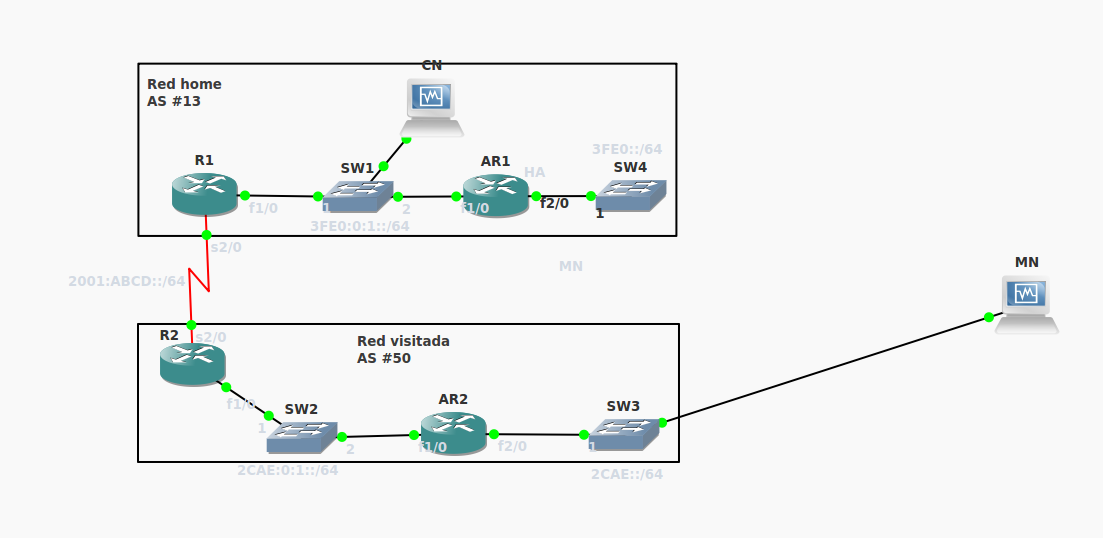
\includegraphics[scale=0.4]{images/topdesc.png}
\end{center}

Observamos en la salida de \textit{ping6} (ver anexo) que en los primeros mensajes tenemos un tiempo cercano a los 20ms de respuesta, y en el mensaje \textit{icmp\_seq=35} pasamos a tiempos de varios cientos, incluso mil milisegundos, y en el proceso hemos perdido el mensaje \textit{icmp\_seq=34}

En el router AR1 podemos ver también el listado de bindings del Home Agent:

\begin{center}
	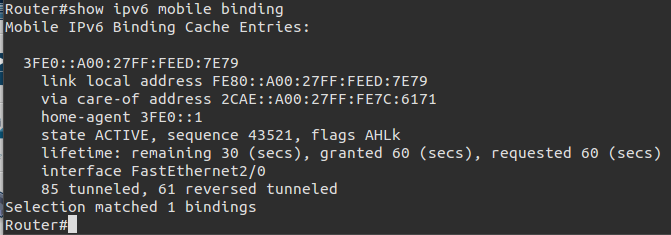
\includegraphics[scale=0.6]{images/ar1binding.png}
\end{center}

Observamos la dirección del Home Address del MN (la dirección a la que hacemos ping6); la Care-of Address, que pertenece a la subred de AR2 a la que está conectado el MN por la interfaz eth2; la dirección del Home-Agent, la de AR1 por la interfaz FE2/0 que fijamos antes. También notamos cómo tiene en lifetime un tiempo de 60 segundos de vida para cada binding, los configurados en \textit{mip6d.conf}.

Ahora veamos las trazas capturadas en el corte:

En la captura realizada en AR2 por la interfaz FE2/0 (a la que se conecta el MN) filtramos todos los mensajes \textit{ICMPv6} y vemos que el primer ping que se registra es el \textit{icmp\_seq=35} en la traza 94, que le llega al CN con un ping de 410ms. Ahora filtramos por \textit{mipv6} y vemos que en las trazas 90 y 93 están los mensajes de binding update y binding ack correspondientes al corte, justo antes del primer mensaje de ping. Además en las trazas 292 y 295 tenemos otro par de mensajes de binding que coinciden por la marca de tiempo a la caducidad de un minuto de cada binding.



\begin{center}
	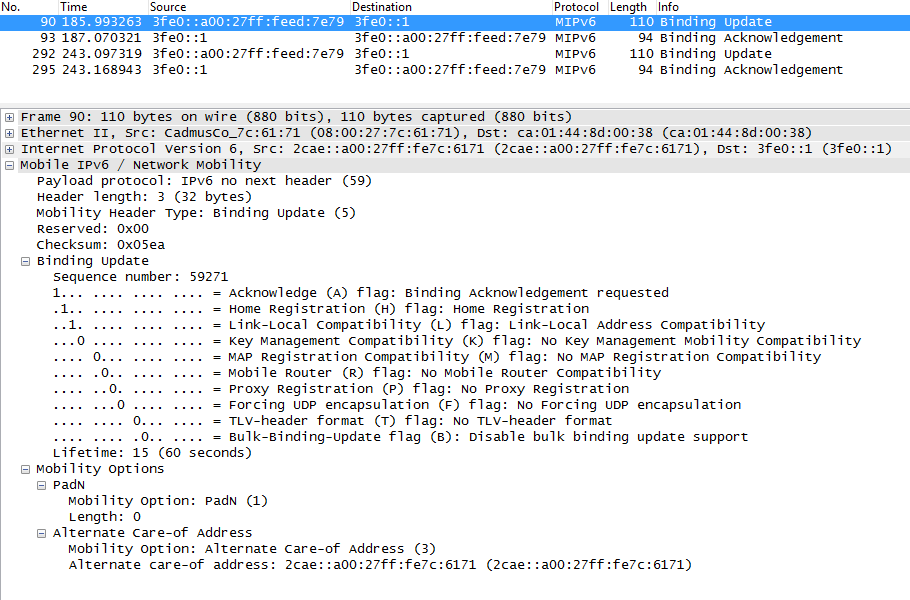
\includegraphics[scale=0.7]{images/bindUpdate.PNG}
\end{center}

\begin{center}
	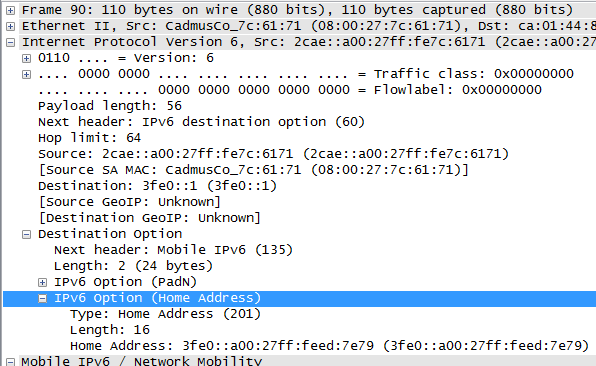
\includegraphics[scale=0.7]{images/bindDestOpt.PNG}
\end{center}

La imagen anterior es el primer binding update que manda el MN y vemos que el origen real del paquete IPv6 es de la subred 2CAE::/64, de AR2, la red visitada, pero tiene una destination option de tipo \textit{home address} que indica al home agent que su dirección Home Adress es la 3fe0::a00:27ff:feed:7e79. Así en la lista de trazas la fuente del mensaje parece que es de la subred 3FE0::/64 pero en verdad es de 2CAE::/64.

En la imagen del Destination Option vemos que el campo Next Header indica MobileIPv6, y en dicha cabecera, como ya no hay más, indica IPv6 no next header.

En cuanto al mensaje de Binding Update en sí, vemos que en los flags tiene activados el de ACK requested, obligatorio en cualquier Binding Update, el flag de Home Registration, pues el mensaje va destinado al Home Agent para que le reenvíe los mensajes al CoA. Notamos también que el flag K está a cero porque hemos desactivado la seguridad con IPsec, por lo que no tiene información de IKE que mantener entre cambios de IP. Tras los flags vemos que el tiempo de vida del binding es el configurado de 60 segundos.

La dirección Care-of Address la indica en la opción \textit{Alternate Care-of Address} y vemos que es la misma que la IPsrc del paquete IPv6, de la subred 2CAE::/64.

\begin{center}
	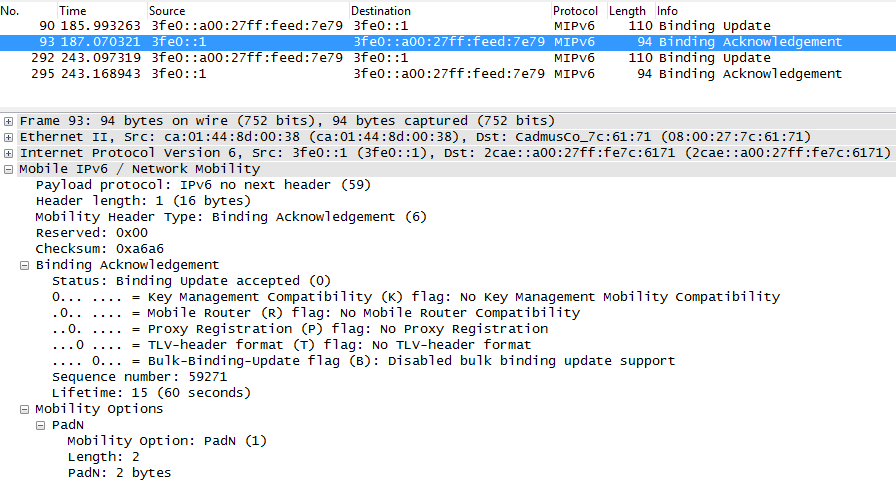
\includegraphics[scale=0.7]{images/bindACK.PNG}
\end{center}

\begin{center}
	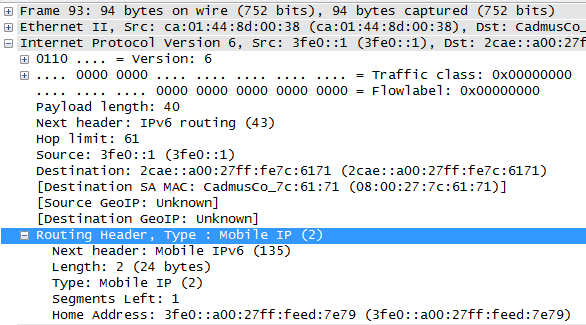
\includegraphics[scale=0.7]{images/bindRoutHead.PNG}
\end{center}

En las imágenes de la traza 93 vemos que se trata de un Binding ACK exitoso, sin mucha más información interesante por parte del binding ack, pero sí por parte de las cabeceras IPv6 previas, pues le precede una Routing Header de tipo 2, con información de la Home Address, de ahí que en el listado de trazas aparezca como dirección de destino la Home Address, mientras que el paquete IPv6 está realmente dirigido a la Care-of Address en 2CAE::/64.



Finalmente volvemos a unir el cable de eth1 con AR1. Se pierden varios mensajes, casi 50, y en el 154 nos contestan \textit{destino inalcanzable}. Finalmente, en el mensaje 155 volvemos a recibir respuesta y además con un ping cercano a los 20ms iniciales.

\begin{center}
	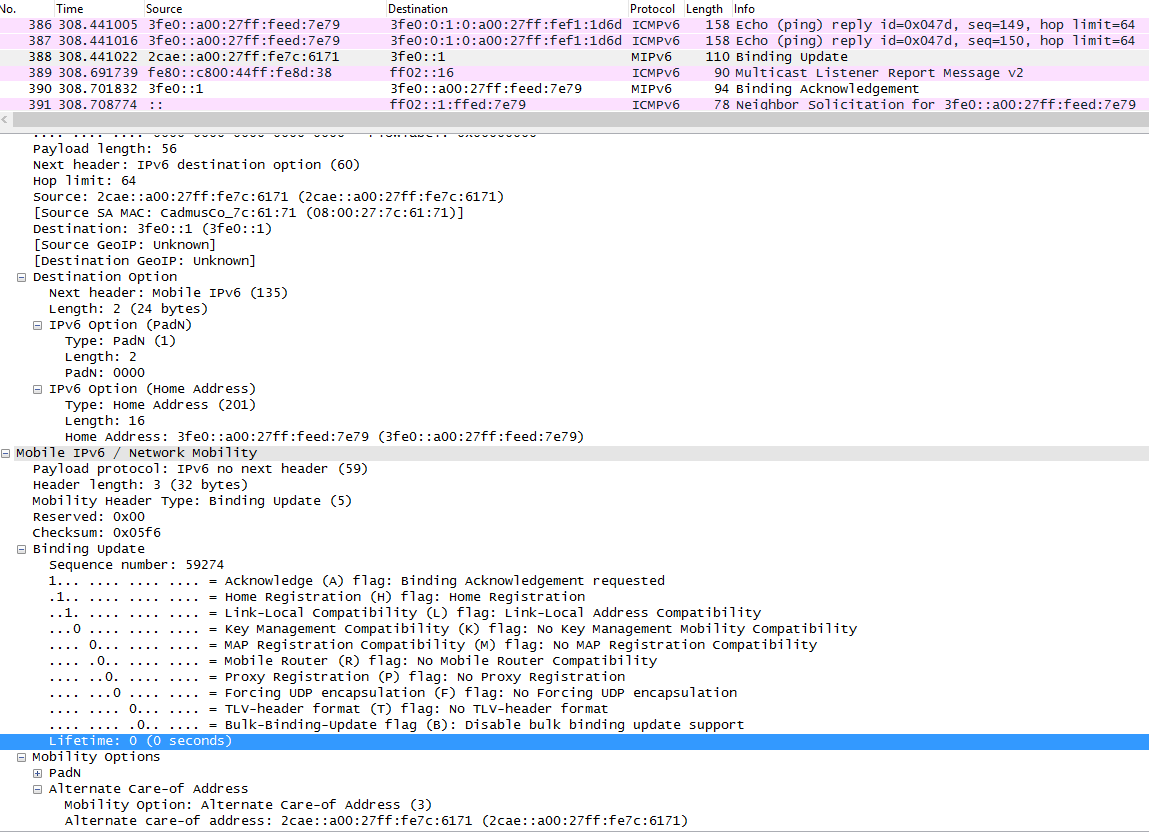
\includegraphics[scale=0.6]{images/bindEND.PNG}
\end{center}


En las trazas tomadas en AR1 vemos que existen únicamente dos mensajes MIPv6, y justo cuando vuelven a aparecer mensajes de ping con números de secuencia a partir del 149.

En la cabecera IPv6 vemos de nuevo el Destination Option con la Home Address, y en el binding update la información es la misa que en el analizado antes, exceptuando el Lifetime del binding, que es 0, de modo que en el Home Agent se elimina y los paquetes destinados al MN se le envían directamente de nuevo.



\section{Traceroute6 CN\texorpdfstring{$\rightarrow$}MN}

En la prueba de antes hacíamos ping, cortábamos el cable, y volvíamos a unirlo, mientras que el ping6 seguía funcionando. Ahora iniciamos con ping6, cortamos el cable, comprobamos que la movilidad funciona, y ejecutamos sin volver a unir el cable:

\begin{BVerbatim}
traceroute6 3fe0::a00:27ff:feed:7e79
\end{BVerbatim}

En la salida del comando observamos que llega un primer salto a la interfaz de AR1 en la subred del CN, y en la segunda entrada AR1 contesta por la misma interfaz que no hay host, es decir, que no está la máquina MN. Ante estos resultados inesperados, he repetido la prueba numerosas veces comprobando que las MACs de las máquinas virtuales no son las mismas, pues se reinicializaron en la clonación, que no tienen la misma IPv6, y además, ejecutando alternamente las órdenes de ping6 y traceroute6 desde el CN al MN con el cable cortado, la respuesta de traceroute es siempre la misma, y ping6 funciona sin problemas con la movilidad. En los adjuntos estás las trazas con las capturas de dichas pruebas que muestran cómo AR1 devuelve un mensaje de Time Exceeded: hop limit exceeded in transit con el primer mensaje (lo esperado de traceroute para detectar el primer salto), y un Destination Unreacheable: Address unreacheable, con la contestación al segundo mensaje de hop limit = 2.

En las trazas tomadas en AR2 se observa que al MN le llegan varios bloques de mensajes ping6, que corresponden con los realizados pues al alternar entre ping6 y traceroute6 sólo dejábamos 4 mensajes, y en las trazas van del seq=1 al seq=4 en varios bloques seguidos. Sin embargo, esos mismos bloques de ping en AR1 están intercalados por los mensajes UDP y de error anteriores.

Los mensajes UDP son los request de traceroute, pues la técnica por defecto de la implementación es enviar a puertos que tienen poca probabilidad de estar en escucha por una aplicación, un mensaje con destino el pedido y hop limit cada vez mayor. Para descartar que sea el uso de UDP el responsable de este error, usamos el comando traceroute -6 -I, y traceroute -6 -T que en vez de usar UDP, usan ICMP y TCP respectivamente, pero los resultados son los mismos.

Podemos concluir que existe algún error con el router Cisco usado, donde el ping funciona perfectamente pero el traceroute que llega a un MN con binding falla, pues cuando está conectado por cable el MN a AR1, todo funciona bien.

En el caso de que todo hubiera funcionado, el resultado esperado es que el traceroute mostrara al MN a 2 saltos, CN a AR1, AR1 a MN, debido a que el HA y el MN hacen encapsulación IPv6 a los mensajes, que se puede verificar en los PING capturados en AR2.

Una captura del resultado que se obtiene con el comando en todas las pruebas:


\begin{center}
	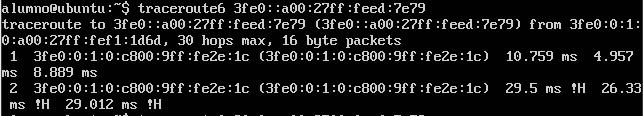
\includegraphics[scale=0.6]{images/trac6.png}
\end{center}



\section{Análisis opcional Neighbour Discovery}
A continuación analizo dos mensajes de neighbour solicitation tomados en la interfaz FE2/0 de AR1:

Neighbor Solicitation:

\begin{center}
	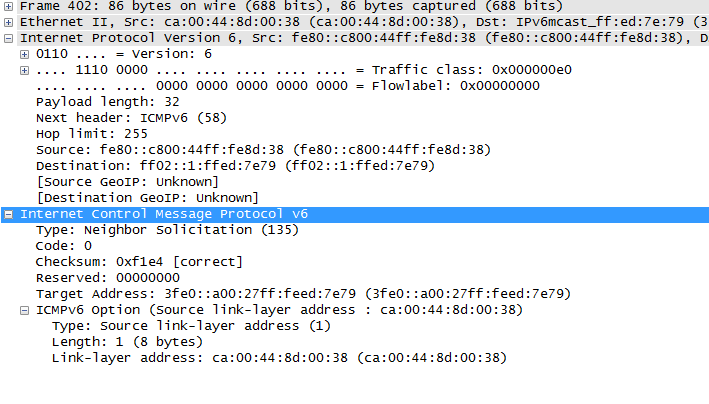
\includegraphics[scale=0.8]{images/neighSol.PNG}
\end{center}

En el paquete IPv6 vemos que el next header es el ICMPv6 de Neighbor Solicitation, el hop limit está a 255 para comprobar que no sale del tramo de red en el que se envía, se conoce la IP propia (source) y se pregunta por una dirección multicast, que por terminar en 1:ffed:7e79 es la Solicited Node Multicast Address del MN. El origen del paquete corresponde a la dirección Link-Local de AR1, que se puede comprobar por su MAC en el último mensaje de Binding ACK visto (origen 3FE0::1).

En el mensaje ICMP en sí vemos que tiene el campo de Target Address con la dirección del MN, y como campo option adicional, el Source Link-Layer address, la dirección MAC origen de AR1 que solicita el Neighbor Advertisement.


\hfill

\hfill

Neighbor Advertisement:

\begin{center}
	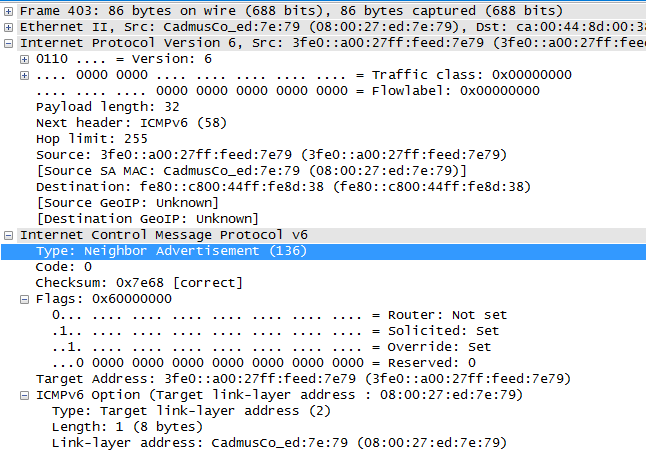
\includegraphics[scale=0.8]{images/neighAdv.PNG}
\end{center}

Aquí tenemos la contestación al NS anterior. En la cabecera IPv6 vemos que el next-header es un ICMPv6, el hop limit es 255 igual que antes, y las direcciones de fuente y destino son ahora unicast, ya no se usa la multicast de Solicited Node. En concreto la IP fuente es global y la destino es link-local.

En el mensaje ICMPv6 tenemos en los flags que no es un router (es el MN en concreto), que el Advertisement es solicitado (por eso no lo envía a All-Nodes), y que se deben reescribir las entradas de las cachés con la nueva información.

Añade el Target Address con la dirección pedida del MN, y una Option con el Target Link-Layer Address, la MAC de la interfaz eth1 del MN. Esta información al final del proceso es la equivalente a la que conseguiría con ARP e IPv4.


\appendix
\section{Ping6 salida por pantalla}
\begin{Verbatim}
PING 3fe0::a00:27ff:feed:7e79(3fe0::a00:27ff:feed:7e79)
from 3fe0:0:1:0:a00:27ff:fef1:1d6d eth1: 56 data bytes
64 bytes from 3fe0::a00:27ff:feed:7e79: icmp_seq=1 ttl=63 time=44.3 ms
64 bytes from 3fe0::a00:27ff:feed:7e79: icmp_seq=2 ttl=63 time=17.1 ms
64 bytes from 3fe0::a00:27ff:feed:7e79: icmp_seq=3 ttl=63 time=20.8 ms
64 bytes from 3fe0::a00:27ff:feed:7e79: icmp_seq=4 ttl=63 time=14.8 ms
64 bytes from 3fe0::a00:27ff:feed:7e79: icmp_seq=5 ttl=63 time=18.6 ms
64 bytes from 3fe0::a00:27ff:feed:7e79: icmp_seq=6 ttl=63 time=22.0 ms
64 bytes from 3fe0::a00:27ff:feed:7e79: icmp_seq=7 ttl=63 time=15.4 ms
64 bytes from 3fe0::a00:27ff:feed:7e79: icmp_seq=8 ttl=63 time=19.4 ms
64 bytes from 3fe0::a00:27ff:feed:7e79: icmp_seq=9 ttl=63 time=22.8 ms
64 bytes from 3fe0::a00:27ff:feed:7e79: icmp_seq=10 ttl=63 time=16.5 ms
64 bytes from 3fe0::a00:27ff:feed:7e79: icmp_seq=14 ttl=63 time=17.3 ms
64 bytes from 3fe0::a00:27ff:feed:7e79: icmp_seq=15 ttl=63 time=20.5 ms
64 bytes from 3fe0::a00:27ff:feed:7e79: icmp_seq=16 ttl=63 time=23.6 ms
64 bytes from 3fe0::a00:27ff:feed:7e79: icmp_seq=17 ttl=63 time=15.3 ms
64 bytes from 3fe0::a00:27ff:feed:7e79: icmp_seq=18 ttl=63 time=18.0 ms
64 bytes from 3fe0::a00:27ff:feed:7e79: icmp_seq=19 ttl=63 time=20.9 ms
64 bytes from 3fe0::a00:27ff:feed:7e79: icmp_seq=20 ttl=63 time=22.1 ms
64 bytes from 3fe0::a00:27ff:feed:7e79: icmp_seq=21 ttl=63 time=14.0 ms
64 bytes from 3fe0::a00:27ff:feed:7e79: icmp_seq=22 ttl=63 time=16.9 ms
64 bytes from 3fe0::a00:27ff:feed:7e79: icmp_seq=23 ttl=63 time=18.9 ms
64 bytes from 3fe0::a00:27ff:feed:7e79: icmp_seq=24 ttl=63 time=21.5 ms
64 bytes from 3fe0::a00:27ff:feed:7e79: icmp_seq=25 ttl=63 time=23.6 ms
64 bytes from 3fe0::a00:27ff:feed:7e79: icmp_seq=26 ttl=63 time=16.0 ms
64 bytes from 3fe0::a00:27ff:feed:7e79: icmp_seq=27 ttl=63 time=19.3 ms
64 bytes from 3fe0::a00:27ff:feed:7e79: icmp_seq=28 ttl=63 time=22.9 ms
64 bytes from 3fe0::a00:27ff:feed:7e79: icmp_seq=29 ttl=63 time=15.9 ms
64 bytes from 3fe0::a00:27ff:feed:7e79: icmp_seq=30 ttl=63 time=18.0 ms
64 bytes from 3fe0::a00:27ff:feed:7e79: icmp_seq=31 ttl=63 time=21.3 ms
64 bytes from 3fe0::a00:27ff:feed:7e79: icmp_seq=32 ttl=63 time=13.9 ms
64 bytes from 3fe0::a00:27ff:feed:7e79: icmp_seq=33 ttl=63 time=17.2 ms
64 bytes from 3fe0::a00:27ff:feed:7e79: icmp_seq=35 ttl=63 time=410 ms
64 bytes from 3fe0::a00:27ff:feed:7e79: icmp_seq=36 ttl=63 time=1067 ms
64 bytes from 3fe0::a00:27ff:feed:7e79: icmp_seq=37 ttl=63 time=198 ms
64 bytes from 3fe0::a00:27ff:feed:7e79: icmp_seq=38 ttl=63 time=202 ms
64 bytes from 3fe0::a00:27ff:feed:7e79: icmp_seq=39 ttl=63 time=247 ms
64 bytes from 3fe0::a00:27ff:feed:7e79: icmp_seq=40 ttl=63 time=583 ms
64 bytes from 3fe0::a00:27ff:feed:7e79: icmp_seq=41 ttl=63 time=1060 ms
64 bytes from 3fe0::a00:27ff:feed:7e79: icmp_seq=42 ttl=63 time=1066 ms
64 bytes from 3fe0::a00:27ff:feed:7e79: icmp_seq=43 ttl=63 time=1071 ms
64 bytes from 3fe0::a00:27ff:feed:7e79: icmp_seq=44 ttl=63 time=1064 ms
64 bytes from 3fe0::a00:27ff:feed:7e79: icmp_seq=45 ttl=63 time=807 ms
64 bytes from 3fe0::a00:27ff:feed:7e79: icmp_seq=46 ttl=63 time=1063 ms
64 bytes from 3fe0::a00:27ff:feed:7e79: icmp_seq=47 ttl=63 time=197 ms
64 bytes from 3fe0::a00:27ff:feed:7e79: icmp_seq=48 ttl=63 time=244 ms
64 bytes from 3fe0::a00:27ff:feed:7e79: icmp_seq=49 ttl=63 time=1062 ms
64 bytes from 3fe0::a00:27ff:feed:7e79: icmp_seq=50 ttl=63 time=845 ms
64 bytes from 3fe0::a00:27ff:feed:7e79: icmp_seq=51 ttl=63 time=86.1 ms
64 bytes from 3fe0::a00:27ff:feed:7e79: icmp_seq=52 ttl=63 time=1075 ms
64 bytes from 3fe0::a00:27ff:feed:7e79: icmp_seq=53 ttl=63 time=1073 ms
64 bytes from 3fe0::a00:27ff:feed:7e79: icmp_seq=54 ttl=63 time=1067 ms
64 bytes from 3fe0::a00:27ff:feed:7e79: icmp_seq=55 ttl=63 time=1062 ms
64 bytes from 3fe0::a00:27ff:feed:7e79: icmp_seq=56 ttl=63 time=172 ms
64 bytes from 3fe0::a00:27ff:feed:7e79: icmp_seq=57 ttl=63 time=177 ms
64 bytes from 3fe0::a00:27ff:feed:7e79: icmp_seq=58 ttl=63 time=222 ms
64 bytes from 3fe0::a00:27ff:feed:7e79: icmp_seq=59 ttl=63 time=1082 ms
64 bytes from 3fe0::a00:27ff:feed:7e79: icmp_seq=60 ttl=63 time=817 ms
64 bytes from 3fe0::a00:27ff:feed:7e79: icmp_seq=61 ttl=63 time=1074 ms
64 bytes from 3fe0::a00:27ff:feed:7e79: icmp_seq=62 ttl=63 time=1071 ms
64 bytes from 3fe0::a00:27ff:feed:7e79: icmp_seq=63 ttl=63 time=1066 ms
64 bytes from 3fe0::a00:27ff:feed:7e79: icmp_seq=64 ttl=63 time=1071 ms
64 bytes from 3fe0::a00:27ff:feed:7e79: icmp_seq=65 ttl=63 time=975 ms
64 bytes from 3fe0::a00:27ff:feed:7e79: icmp_seq=66 ttl=63 time=1072 ms
64 bytes from 3fe0::a00:27ff:feed:7e79: icmp_seq=67 ttl=63 time=155 ms
64 bytes from 3fe0::a00:27ff:feed:7e79: icmp_seq=68 ttl=63 time=200 ms
64 bytes from 3fe0::a00:27ff:feed:7e79: icmp_seq=69 ttl=63 time=1070 ms
64 bytes from 3fe0::a00:27ff:feed:7e79: icmp_seq=70 ttl=63 time=194 ms
64 bytes from 3fe0::a00:27ff:feed:7e79: icmp_seq=71 ttl=63 time=1074 ms
64 bytes from 3fe0::a00:27ff:feed:7e79: icmp_seq=72 ttl=63 time=790 ms
64 bytes from 3fe0::a00:27ff:feed:7e79: icmp_seq=73 ttl=63 time=191 ms
64 bytes from 3fe0::a00:27ff:feed:7e79: icmp_seq=74 ttl=63 time=1059 ms
64 bytes from 3fe0::a00:27ff:feed:7e79: icmp_seq=75 ttl=63 time=984 ms
64 bytes from 3fe0::a00:27ff:feed:7e79: icmp_seq=76 ttl=63 time=1080 ms
64 bytes from 3fe0::a00:27ff:feed:7e79: icmp_seq=77 ttl=63 time=121 ms
64 bytes from 3fe0::a00:27ff:feed:7e79: icmp_seq=78 ttl=63 time=175 ms
64 bytes from 3fe0::a00:27ff:feed:7e79: icmp_seq=79 ttl=63 time=1074 ms
64 bytes from 3fe0::a00:27ff:feed:7e79: icmp_seq=80 ttl=63 time=769 ms
64 bytes from 3fe0::a00:27ff:feed:7e79: icmp_seq=81 ttl=63 time=1075 ms
64 bytes from 3fe0::a00:27ff:feed:7e79: icmp_seq=82 ttl=63 time=1074 ms
64 bytes from 3fe0::a00:27ff:feed:7e79: icmp_seq=83 ttl=63 time=1070 ms
64 bytes from 3fe0::a00:27ff:feed:7e79: icmp_seq=84 ttl=63 time=1067 ms
64 bytes from 3fe0::a00:27ff:feed:7e79: icmp_seq=85 ttl=63 time=1072 ms
64 bytes from 3fe0::a00:27ff:feed:7e79: icmp_seq=86 ttl=63 time=311 ms
64 bytes from 3fe0::a00:27ff:feed:7e79: icmp_seq=87 ttl=63 time=94.3 ms
64 bytes from 3fe0::a00:27ff:feed:7e79: icmp_seq=88 ttl=63 time=137 ms
64 bytes from 3fe0::a00:27ff:feed:7e79: icmp_seq=89 ttl=63 time=111 ms
64 bytes from 3fe0::a00:27ff:feed:7e79: icmp_seq=90 ttl=63 time=97.1 ms
64 bytes from 3fe0::a00:27ff:feed:7e79: icmp_seq=91 ttl=63 time=92.0 ms
64 bytes from 3fe0::a00:27ff:feed:7e79: icmp_seq=92 ttl=63 time=187 ms
From 3fe0:0:1:0:c800:44ff:fe8d:1c icmp_seq=154 Destination unreachable: Address unreachable
64 bytes from 3fe0::a00:27ff:feed:7e79: icmp_seq=155 ttl=63 time=21.6 ms
64 bytes from 3fe0::a00:27ff:feed:7e79: icmp_seq=156 ttl=63 time=14.4 ms
64 bytes from 3fe0::a00:27ff:feed:7e79: icmp_seq=157 ttl=63 time=18.3 ms
64 bytes from 3fe0::a00:27ff:feed:7e79: icmp_seq=158 ttl=63 time=21.4 ms
64 bytes from 3fe0::a00:27ff:feed:7e79: icmp_seq=159 ttl=63 time=14.5 ms
64 bytes from 3fe0::a00:27ff:feed:7e79: icmp_seq=160 ttl=63 time=17.5 ms
64 bytes from 3fe0::a00:27ff:feed:7e79: icmp_seq=161 ttl=63 time=21.1 ms
64 bytes from 3fe0::a00:27ff:feed:7e79: icmp_seq=162 ttl=63 time=14.9 ms
64 bytes from 3fe0::a00:27ff:feed:7e79: icmp_seq=163 ttl=63 time=17.3 ms
64 bytes from 3fe0::a00:27ff:feed:7e79: icmp_seq=164 ttl=63 time=20.2 ms
64 bytes from 3fe0::a00:27ff:feed:7e79: icmp_seq=165 ttl=63 time=13.2 ms
64 bytes from 3fe0::a00:27ff:feed:7e79: icmp_seq=166 ttl=63 time=16.4 ms
64 bytes from 3fe0::a00:27ff:feed:7e79: icmp_seq=167 ttl=63 time=19.9 ms
64 bytes from 3fe0::a00:27ff:feed:7e79: icmp_seq=168 ttl=63 time=22.2 ms
64 bytes from 3fe0::a00:27ff:feed:7e79: icmp_seq=169 ttl=63 time=15.2 ms
64 bytes from 3fe0::a00:27ff:feed:7e79: icmp_seq=170 ttl=63 time=18.1 ms
64 bytes from 3fe0::a00:27ff:feed:7e79: icmp_seq=171 ttl=63 time=11.2 ms
64 bytes from 3fe0::a00:27ff:feed:7e79: icmp_seq=172 ttl=63 time=14.8 ms
64 bytes from 3fe0::a00:27ff:feed:7e79: icmp_seq=173 ttl=63 time=16.6 ms
64 bytes from 3fe0::a00:27ff:feed:7e79: icmp_seq=174 ttl=63 time=18.0 ms
64 bytes from 3fe0::a00:27ff:feed:7e79: icmp_seq=175 ttl=63 time=21.2 ms
64 bytes from 3fe0::a00:27ff:feed:7e79: icmp_seq=176 ttl=63 time=14.8 ms
64 bytes from 3fe0::a00:27ff:feed:7e79: icmp_seq=177 ttl=63 time=17.2 ms
64 bytes from 3fe0::a00:27ff:feed:7e79: icmp_seq=178 ttl=63 time=20.1 ms
64 bytes from 3fe0::a00:27ff:feed:7e79: icmp_seq=179 ttl=63 time=13.3 ms
64 bytes from 3fe0::a00:27ff:feed:7e79: icmp_seq=180 ttl=63 time=15.8 ms
\end{Verbatim}



\begin{thebibliography}{99}
	\bibitem{apuntes}
	Apuntes

	%TODO
\end{thebibliography}


\end{document}
